\documentclass[a4paper]{jpconf}
\usepackage[utf8]{inputenc}

\usepackage{graphicx} % Required for including pictures
\usepackage{listings}
\usepackage{float} % Allows putting an [H] in \begin{figure} to specify the exact location of the figure
\usepackage{wrapfig} % Allows in-line images such as the example fish picture
\usepackage{color}


\begin{document}


% Title Page
\title{
DPM Evolution: a Disk Operations Management Engine for DPM}

\author{Andrea Manzi, Fabrizio Furano, Oliver Keeble, Georgios Bitzes}

\address{CERN IT}

\ead{amanzi@cern.ch, furano@cern.ch, okeeble@cern.ch, georgios.bitzes@cern.ch}

\begin{abstract}

The DPM (Disk Pool Manager) project is the most widely deployed solution for storage of
large data repositories on Grid sites, and is completing the most important upgrade
in its history, with the aim of bringing important new features, performance
and easier long term maintainability.
Work has been done to make the so-called "legacy stack" optional, and substitute
it with an advanced implementation that is based on the fastCGI and RESTful technologies.
Beside the obvious gain in making optional several legacy components that
are difficult to maintain, this step brings important features together with
performance enhancements. Among the most important features we can cite the
simplification of the configuration, the possibility of working in a totally
SRM-free mode, the implementation of quotas, free/used space on directories,
and the implementation of volatile pools that can pull files from external
sources, which can be used to deploy data caches.
Moreover, the communication with the new core, called DOME
(Disk Operations Management Engine) now happens through secure HTTPS channels
through an extensively documented, industry-compliant protocol.
For this leap, referred to with the codename "DPM Evolution", the help of the
DPM collaboration has been very important in the beta testing phases,
and here we report about the technical choices.

\end{abstract}



\newpage % Begins the essay on a new page instead of on the same page as the table of contents


%----------------------------------------------------------------------------------------
%	TABLE OF CONTENTS
%----------------------------------------------------------------------------------------

\section{Introduction}
The Disk Pool Manager (DPM) is a lightweight solution for grid enabled disk storage
management. Operated at around 150 sites, it has the widest distribution of all grid storage
solutions in the WLCG infrastructure, and in total it manages around 70PB of data. DPM provides
an easy way to manage and configure disk pools, and exposes multiple interfaces for
data access (xrootd, GridFTP and HTTP/WebDAV) and control (SRM).\\
The development direction of the last years has been towards simplifying the
system, while supporting all the advanced features that are needed by the Grid computing and
helping sites to incrementally renew their setups.
This effort is also dictated by the difficulty of maintaining software libraries that have been
written in the 80s and 90s, over which the oldest core components of DPM are based.\\
Work had been done in the last years to create the \textit{dmlite} \cite{dpmfuture} framework and a set of plugins
that started complementing the core features of DPM by giving support for the more recent
data access protocols used by HEP (\textit{HTTP with multi-range requests} and \textit{xrootd}),
while keeping the older core components as an internal coordination layer that includes
support for the SRM protocols.\\
The development cycle that ended in Q4/2016 has successfully removed this functional
dependency, making the usage of the older components optional, and linked to the
foreseen phase-out of the usage of the SRM protocol in the Grid. This was accomplished by
writing a brand new core component that acts as coordination layer and can coexist with the
older one in various ways.


\section{DOME}

DOME (Disk operations Management Engine) is a robust, high performance server that manages the operations of a DPM cluster. DOME is built on the \textit{FastCGI} \cite{fastcgi} technology,
and uses HTTP and JSON to communicate with clients.
The adoption of DOME aims at augmenting the Disk Pool Manager (DPM) system so that its core coordination functions and inter-cluster communication paths are
implemented through open components, and following contemporary development approaches headed to performance, scalability and maintainability. We can summarize the
main goals of DOME as:

\begin{itemize}
 \item Making optional all the so-called legacy components that are provided by the \textit{lcg-dm} code tree, namely \textit{libshift}, \textit{rfiod},
 \textit{dpm(daemon)}, \textit{dpnsdaemon}, \textit{CSec} and others.
 \item provide a software infrastructure where adding new coordination features is easier than with the historical one
 \item provide full support for asynchronous calculation of file checksums of multiple types
 \item provide support for checking the consistence of replicas through their checksums
 \item provide structure, hooks and callouts that allow the usage of DPM disk pools as large \textit{file caches}
 \item having a unified configuration file that is readable and synthetic, as opposed to the previous approach of having several
 sparse configuration files, all with differently over-simplified syntax rules (or no syntax at all, e.g. \textit{/etc/NSCONFIG})
\end{itemize}

The DOME component has the shape of a \textit{fastCGI} daemon, and has to be triggered by the Apache instances running in the DPM head node and
in all the DPM disk servers. A configuration option defines whether it is running as head node or disk server.

Architecurally speaking, DOME is primarily a service provider for the \textit{dmlite} framework, through a new dmlite plugin called \textit{DOMEAdapter}.\\

\section{DOME: Main features}
DOME has two modalities: \textit{headnode} and \textit{disknode}, which respectively represent
simplified evolutions of the \textit{dpm} daemon and of \textit{rfiod}, together with \textit{libshift} and \textit{Csec}.
The functionalities are roughly as follows:
\begin{itemize}
 \item headnode: general coordination function
 \subitem spreads load (PUT, GET, checksums) towards the available disk nodes
 \subitem keeps an in memory status of the DPM disk/pool topology with disk sizes and free space
 \subitem keeps an in memory status of the ongoing asynchronous checksum calculations
 \subitem keeps an in memory status of the ongoing asynchronous file callouts
 \subitem queues and dispatches to disk nodes the requests for asynchronous checksum calculations that have to be delayed for load balancing reasons
 \subitem queues and dispatches to disk nodes the requests for asynchronous file callouts that have to be delayed for load balancing reasons

 \item disknode: local disk and space-related services
 \subitem Allows to \textit{stat} individual physical files and directories
 \subitem Allows to \textit{statfs} filesystems to get used and free space
 \subitem Allows the local submission of checksum calculations
 \subitem Allows the local submission of file callouts
\end{itemize}

The historical data tunnelling features provided by the \textit{rfio} infrastructure (and used by gridftp in some boundary scenarios) \cite{rfio}
is implemented by DOMEAdapter directly on the top of HTTPS, hence namely it does not use the DOME server.\\

The main difference from the legacy components is that DOME does not apply user authorization again for individual internal
transactions, as the task of authenticating/authorizing remote users is already accomplished by the dmlite frontends.
DOME instead checks that the sender of a request (e.g. a disk server) is authorized to
send requests. DOME applies strong, industry standard authentication protocols to this task.\\
Authentication in DOME is zero-config for the regular cases (one head node and multiple disk servers), and flexible enough
to add arbitrary identities that will be allowed to send commands to it.\\
The activity of DOME is not linked to any particular data access protocol. Its concepts of logical file name and physical file name are not linked to a particular data/metadata transfer protocol.


\subsection{From spacetokens to quota tokens}
Historically, DPM manages space accounting through a set of individual named space reservations that are associated to pools. This follows the
philosophy of the SRM specification \cite{srm}.\\
Semantically, SRM space reservations are named reservations of a part of the space of a disk pool. When  writing data
in workflows that involve SRM, requests to write a replica specify a pool
that has to host the replica, hence ultimately the replica will be subject to the space reservations.\\

One of the weakest points in this schema is that the remote client willing to write a file
has to know the name of a suitable space reservation in the destination system, to be able to write
and be properly accounted for. This information represents a technical detail
of the destination storage, and it can also  be provided wrongly, for example accounting
a file into the wrong spacetoken (e.g. "scratch" versus "production").\\

Another related, historical weak point of this workflow is that calculating precise results for the space occupancies can be a challenging exercise,
especially if the structure of the pools has been modified in the years, following additions of new storage space or
even failures.\\
DOME models an evolution of this mechanism towards \textit{subdirectory-based space accounting}, instead than pool-based, in a way
that is compatible with the older one and can coexist with it.\\

When considering subdirectory-based space accounting, every subdirectory at less than N levels from the root is kept
updated with the total size of the replicas of files that reside in that directory subtree.
This \textit{subdirectory size} together with the information on free/used space in the pools associated to these subdirectory tree
can then be used to compute the needed space occupancy numbers.\\

DOME uses the records describing spacetokens that are kept in the head node DB with minimal modification. Their meaning is slightly changed,
into semantically representing a quota on one and only one directory subtree. From this point on, we will refer to them as \textit{quotatokens},
whose behavior is similar to that of an old spacetoken associated to a directory.\\

A \textit{quotatoken} attached to a directory subtree \textbf{overrides others that may be attached to its parents}.\\
If a directory content (counting all the replicas) exceeds the quota specified by the quotatoken that influences it,
then new PUT requests on that directory will be denied.\\

As a summary, the meaning of a quotatoken specifying a quota of N terabytes on pool X, associated to directory "/dir1" is \textit{use pool X as
space for hosting the files that will be written into \/dir1. Do not allow more than N terabytes to be hosted there}.\\

\subsection{Open checksumming}
DOME supports requests for checksums of arbitrary kind. It can:\\

\begin{itemize}
 \item return the corresponding checksum that is stored in the name space
 \item choose an appropriate replica of the file and tell to the disk node managing it to calculate its checksum
 \item force the recalculation of the checksum and store it into the name space
\end{itemize}

The checksum calculation requests are queued in the head node, in memory. The architecture of the queue
is designed to be self-healing in the case the checksum calculations do not end correctly, or some machines are restarted,
including the head node itself.


\section{Architecture}
Figure \ref{figdomedisk} shows the main components of DOME that are in action in a disk server.\\
Requests come through Apache already authenticated and referring to the two possible paths that
are associated either to the filesystems or to the dome command path which starts with \lstinline{/domedisk}.
Another detail that characterizes a disk server for DOME is the ability to execute tasks like checksum calculations
and file pulls from external sources. These tasks, following a logic that is based on time, report their status
to the head node, which uses this information to keep its queues updated.\\
 
\begin{figure}
\begin{center}
 \includegraphics[width=10cm,keepaspectratio=true,angle=-90,origin=c]{./pics/domepics_disk.eps}
 % domepics_disk.ps: 0x0 pixel, 300dpi, 0.00x0.00 cm, bb=
 \caption{Simplified diagram of DOME in a disk node}
 \label{figdomedisk}
\end{center}
\end{figure}

A DOME head node is slightly more complex than a disk server, and its internal structure is
visible in Figure \ref{figdomehead}.\\
Requests come through Apache already authenticated and referring to the two possible paths that
refer either to the logical name space ( \lstinline{/dpm} ) or to the dome command path which starts with \lstinline{/domehead}.
A head node can contact external systems to get information about remote files, and queues in memory the requests for checksum calculations and remote file pulling.\\


\begin{figure}
\begin{center}
 \includegraphics[width=10cm,keepaspectratio=true,angle=-90,origin=c]{./pics/domepics_head.eps}
 % domepics_disk.ps: 0x0 pixel, 300dpi, 0.00x0.00 cm, bb=
 \caption{Simplified diagram of DOME in a head node}
 \label{figdomehead}
\end{center}

\end{figure}

\subsection{Checksum queuer}
 DOME internally queues and schedules checksum calculation requests in the head node. We can summarize the applied behaviour as:
 \begin{itemize}
  \item No more than N checksums will be run per disk mount\\
  \item No more than L checksums will be run per disk server\\
  \item No more than M checksums will be run in total\\
 \end{itemize}
 
 Checksum requests are queued in memory and dispatched to suitable disk nodes that become available with respect to the mentioned criteria. The disk nodes instances
 constantly update the head node about the running checksums, hence the system will self-heal on restarts of the head node.\\
 When finished calculating a checksum, a disk node will notify the head node and pass the result (or failure).\\
 
\subsection{File pull queuer}
DOME internally on the head node queues and schedules requests for file pulls from external locations. We can summarize the applied behaviour as:
 \begin{itemize}
  \item No more than N pulls will be run per disk mount\\
  \item No more than L pulls will be run per disk server\\
  \item No more than M pulls will be run in total\\
 \end{itemize}
 
The file pull itself is implemented as a simple callout in the disk server, that can invoke any file movement mechanism.
The pull callout in the disk server is complemented by a stat callout, which is able to get information from
an external system for the presence of an offline file.\\

Pull requests are queued in memory and dispatched to disk nodes that match the request and become available.
The disk nodes instances constantly update the head node on the running callouts, and the system will self-heal
on restarts of the head node. When finished pulling a file, a disk node will notify the head node and pass the result (or failure).\\

\section{Transitioning steps}
As we remarked, the new components are totally compatible with the older ones and can coexist with them, if
properly configured. This has been an important design decision.\\
With this in mind, one can write a reasonably exhaustive set of steps, through which a DPM site will
likely decide to incrementally upgrade their deployments. The goal is to stay up-to-date with the
latest developments and with the features that the LHC experiments ask for, like for example a more reliable
and precise storage accounting scheme.\\
\begin{itemize}
 \item Starting with the release of DPM 1.9 (which includes DOME) that happened in Q4/2017, the sites can start upgrading
head nodes and disk servers at the pace that they prefer. It may be likely that most of the sites will have upgraded
during 2017. At this stage, the features will be the same as before, with the addition of a more powerful \textit{dmlite-shell}.
 \item When the whole cluster has been updated, the administrator can prime the space report counters, following the updated
setup instructions. From this moment on, the site will precisely keep track of the disk space used (not the free space yet).
 \item The next step will be to use the dmlite-shell and associate each of the existing spacetokens to a suitable directory
in the logical name space of the Virtual Organization they belong to.
 \item The successive step is to re-run the configuration step, and notify to the system that it can fully enable
all the features of DOME.
\end{itemize}

When these steps are completed, the system is running both the historical software stack and the new one, at the same time.
All the recent features are enabled, including the ability of producing sophisticated per-directory free/used space reports.\\
At this point the older stack will be used only for SRM services. Once the SRM services are not used anymore, the
system administrator can safely choose to uninstall the older components.




\section{Conclusion}

The introduction of Dome represents the final component in DPM's definitve architecture. The project's
platform for the future has now reached its final shape and foresees just components consolidations.
With a fully modernised, maintainable stack, scaleable architecture
and rich protocol support, DPM is able to protect the investment of the large number of sites who have
entrusted their data to it and can expect to absorb future data volumes without major architectural modifications.


\section*{References}
\begin{thebibliography}{9}

\bibitem{xrdwan} Scalla/xrootd WAN globalization tools: Where we are
Fabrizio Furano and Andrew Hanushevsky 2010 J. Phys.: Conf. Ser. 219 072005
\verb"http://iopscience.iop.org/1742-6596/219/7/072005/"

\bibitem{xrd} The xrootd.org homepage
\verb"http://www.xrootd.org"

\bibitem{dpmfuture} DPM: Future Proof Storage
Alejandro Alvarez, Alexandre Beche, Fabrizio Furano, Martin Hellmich, Oliver Keeble, Ricardo Rocha
CHEP2012

\bibitem{dpmnew} Web enabled data management with DPM \& LFC
Alejandro Alvarez Ayllon, Alexandre Beche, Fabrizio Furano, Martin Hellmich, Oliver Keeble and Ricardo Brito Da Rocha
CHEP2012

\bibitem{fastcgi} Paul Heinlein. 1998. FastCGI. Linux J. 1998, 55es, Article 1 (November 1998).

\bibitem{srm} Storage Resource Management (SRM) Working Group, Storage Resource Management (SRM) Working Group

\bibitem{rfio} R. Kalmady, B. Tierney, A comparison of GSIFTP and RFIO on a WAN, in: Proceedings of CHEP'01, September 3-7, Beijing, China, 2001.
\end{thebibliography}

\end{document}
